\documentclass[UTF8,zihao=-4,scheme=chinese,fontset=mac]{ctexart}

\usepackage[a4paper,top=30mm,bottom=25mm,left=30mm,right=25mm,headheight=15pt,headsep=12pt,footskip=15mm]{geometry}
\usepackage{fontspec}
\usepackage{setspace}
\usepackage{fancyhdr}
\usepackage{titlesec}
\usepackage{titletoc}
\usepackage{tocloft}
\usepackage{graphicx}
\usepackage{booktabs}
\usepackage{longtable}
\usepackage{tabularx}
\usepackage{array}
\usepackage{multirow}
\usepackage{caption}
\usepackage{subcaption}
\usepackage{float}
\usepackage{amsmath}
\usepackage{amssymb}
\usepackage{enumitem}
\usepackage{xcolor}
\usepackage{listings}
\usepackage{hyperref}
\usepackage{url}
\usepackage{ragged2e}
\usepackage{indentfirst}
\usepackage{chngcntr}

\setmainfont{Times New Roman}
\setsansfont{Arial}
\setmonofont{Menlo}
\setCJKmainfont[AutoFakeBold=2.5]{Songti SC}
\setCJKsansfont[AutoFakeBold=2.5]{Heiti SC}
\setCJKmonofont{PingFang SC}
\setCJKfamilyfont{zhsong}[AutoFakeBold=2.5]{Songti SC}
\setCJKfamilyfont{zhhei}[AutoFakeBold=2.5]{Heiti SC}

\hypersetup{
  colorlinks=true,
  linkcolor=black,
  citecolor=black,
  urlcolor=black,
  pdfauthor={霍玮放},
  pdftitle={面向工具调用智能体的安全防火墙Web应用系统设计与实现}
}

\linespread{1.25}
\setlength{\parindent}{2em}
\setlength{\parskip}{0pt}
\renewcommand{\contentsname}{目\quad 录}
\renewcommand{\figurename}{图}
\renewcommand{\tablename}{表}
\renewcommand{\refname}{参考文献}
\counterwithin{figure}{section}
\counterwithin{table}{section}
\counterwithin{equation}{section}

\pagestyle{fancy}
\fancyhf{}
\fancyhead[C]{\zihao{-5}\songti 北京林业大学本科毕业论文}
\fancyfoot[C]{\zihao{5}\thepage}
\renewcommand{\headrulewidth}{0.4pt}

\ctexset{
  section = {
    format = \centering\zihao{3}\bfseries\songti,
    beforeskip = 0.5\baselineskip,
    afterskip = 0.5\baselineskip,
    name = {},
    number = \arabic{section}
  },
  subsection = {
    format = \zihao{4}\bfseries\songti,
    beforeskip = 0.5\baselineskip,
    afterskip = 0.25\baselineskip,
    name = {},
    number = \thesection.\arabic{subsection}
  },
  subsubsection = {
    format = \zihao{-4}\bfseries\songti,
    beforeskip = 0.25\baselineskip,
    afterskip = 0.1\baselineskip,
    name = {},
    number = \thesubsection.\arabic{subsubsection}
  }
}

\captionsetup{
  font={small,bf},
  labelfont=bf,
  labelsep=space,
  justification=centering
}

\renewcommand{\cftsecleader}{\cftdotfill{\cftdotsep}}
\setcounter{tocdepth}{3}

\newcolumntype{Y}{>{\RaggedRight\arraybackslash}X}
\newcolumntype{C}{>{\centering\arraybackslash}X}
\newcommand{\code}[1]{{\ttfamily\small\nolinkurl{#1}}}
\newcommand{\bicaption}[2]{\caption{#1\\\small #2}}
\newcommand{\thesistitlecn}{面向工具调用智能体的安全防火墙Web应用系统设计与实现}
\newcommand{\thesistitleen}{Design and Implementation of a Web-based Agent Firewall for Tool-Calling AI Systems}

\lstset{
  basicstyle=\ttfamily\small,
  breaklines=true,
  frame=single,
  columns=fullflexible,
  keepspaces=true,
  keywordstyle=\color{blue!60!black},
  commentstyle=\color{green!40!black},
  stringstyle=\color{red!60!black},
  showstringspaces=false
}

\begin{document}
\justifying

% -------------------- 封面 --------------------
\begin{titlepage}
  \thispagestyle{empty}
  \centering
  \vspace*{0.5cm}
  {\zihao{4}\songti 学校代码：10022\par}
  \vspace{1.6cm}
  {\zihao{2}\songti\bfseries 本科毕业论文（设计）\par}
  \vspace{1.8cm}
  {\zihao{3}\songti\bfseries \thesistitlecn\par}
  \vspace{0.45cm}
  {\zihao{4}\bfseries \thesistitleen\par}
  \vspace{2.6cm}
  {\zihao{4}\songti 霍玮放\par}
  \vfill
  \begin{tabular}{>{\zihao{4}\songti}p{3.2cm}>{\zihao{4}\songti}p{7.0cm}}
    学\quad 院 & 工学院 \\
    专\quad 业 & 电气工程及其自动化（辅修） \\
    班\quad 级 & 电气24-3 \\
    学\quad 号 & 230206108 \\
    指导教师 & 杨波\quad 教授 \\
  \end{tabular}
  \vfill
  {\zihao{4}\songti 2026年5月\par}
\end{titlepage}

% -------------------- 声明 --------------------
\clearpage
\thispagestyle{empty}
\section*{独创性声明}
本人声明所呈交的论文（设计）是本人在导师指导下独立进行的设计、研究工作及取得的设计、研究成果。尽我所知，除了论文（设计）中特别加以标注和致谢的地方外，论文（设计）中不包含其他人已经发表或撰写过的研究成果，本论文（设计）中没有抄袭他人研究成果和伪造数据等行为。与我共同工作的人员对本研究所做的任何贡献均已在论文（设计）中作了明确的说明并表示了谢意。

\vspace{1.5cm}
\noindent 作者签名：\hspace{5cm} 日期：\hspace{1cm} 年 \hspace{0.5cm} 月 \hspace{0.5cm} 日

\vspace{2.5cm}
\section*{关于毕业论文（设计）使用授权的说明}
本人完全了解北京林业大学有关保留、使用毕业论文（设计）的规定，即：本科生在校期间毕业论文（设计）工作的知识产权单位属北京林业大学；学校有权保留并向国家有关部门或机构送交论文（设计）的纸质版和电子版，允许毕业论文（设计）被查阅、借阅和复印；学校可以将毕业论文（设计）的全部或部分内容公开或编入有关数据库进行检索，可以允许采用影印、缩印或其它复制手段保存、汇编毕业论文（设计）。

\vspace{1.5cm}
\noindent 作者签名：\hspace{4cm} 指导老师签名：\hspace{2cm}

\vspace{0.8cm}
\noindent 日\quad 期：\hspace{1cm} 年 \hspace{0.5cm} 月 \hspace{0.5cm} 日

\clearpage
\thispagestyle{empty}
\section*{AI工具规范使用诚信承诺书}
\subsection*{一、AI工具使用情况说明}
本人郑重声明，在毕业论文（设计）写作过程中使用AI工具的情况如下：

\vspace{0.4cm}
\noindent $\square$ 未使用任何AI工具（勾选此项者无需填写后续内容）

\noindent $\blacksquare$ 使用AI工具（勾选此项者需如实填写以下内容）

\vspace{0.4cm}
\noindent 1. 使用工具名称：ChatGPT、DeepSeek、文献数据库检索工具、LaTeX排版与图表辅助工具。

\noindent 2. 具体用途及生成内容：用于文献检索关键词整理、论文结构草拟、语言润色建议、LaTeX格式调整、图表生成脚本辅助编写。系统设计、实验方案、核心代码理解、数据复核、结论推导由作者结合本项目实际实现独立完成。

\noindent 3. 生成内容占全文比例：\underline{\hspace{1.5cm}} \%（最终提交前由作者据实填写）。

\subsection*{二、诚信承诺}
本人承诺：毕业论文（设计）核心研究内容（包括实验设计、数据分析、结论推导等）均独立完成，未使用AI工具直接生成或替代。上述AI工具使用情况描述真实、准确、完整，无隐瞒或虚假陈述。

\vspace{1.5cm}
\noindent 作者签名：\hspace{5cm} 日期：\hspace{1cm} 年 \hspace{0.5cm} 月 \hspace{0.5cm} 日

% -------------------- 摘要 --------------------
\clearpage
\pagenumbering{Roman}
\setcounter{page}{1}
\section*{摘要}
\addcontentsline{toc}{section}{摘要}

大语言模型驱动的智能体正在从单轮问答系统演进为能够读取外部上下文、调用工具、创建子任务并执行跨系统操作的自动化运行时。OpenClaw、Model Context Protocol（MCP）等协议和框架降低了模型接入工具的成本，但也把传统应用中的权限边界、输入验证、审计追踪和供应链信任问题重新暴露给自然语言接口。提示词注入、间接工具结果注入、越权工具调用、混淆代理、委派链滥用等问题表明，仅依赖模型自身遵循系统提示词不足以构成安全边界。

本研究基于现有 Agent-Firewall 项目，设计并实现了一个面向工具调用智能体的双层安全防火墙Web应用系统。系统由代理防火墙层与智能体运行时防护层组成：代理层以FastAPI和LangGraph构建9节点流水线，在模型调用前后执行解析、意图分类、规则匹配、并行扫描、风险聚合、提示词改写、输出过滤和审计记录；智能体层构建11节点LangGraph运行图，在工具执行前后实施RBAC权限检查、参数Schema验证、注入检测、上下文风险识别、会话限额、敏感工具确认、工具结果PII/密钥清洗和子智能体委派追踪。系统前端采用Nuxt 4与Vuetify实现策略管理、攻击演练、Agent配置、调用链可视化和Trace分析，后端支持Internal、MCP和OpenClaw三类工具提供者。

实验采用离线可复现口径，不依赖真实模型密钥、OpenClaw服务或PostgreSQL。Agent层125个纯内存测试全部通过，覆盖RBAC、前置工具门控、后置输出清洗和Agent图执行。红队基准包含358个场景，其中338个为攻击样本、20个为安全样本；在当前轻量离线环境下，balanced策略检出249个攻击样本，检出率为73.7\%，误报率为0.0\%。仓库历史完整扫描器基准显示，在启用LLM Guard、NeMo Guardrails等完整本地扫描器后，攻击检出率可达97.9\%，同样保持0.0\%误报。本文进一步构造了10类Agent/subagent调用案例，验证系统可对正常订单查询、知识库检索、越权密钥访问、参数注入、外泄上下文、重复失败升级、敏感工具确认、子智能体创建和委派链进行可解释拦截与审计。

研究结果表明，将安全决策从LLM推理闭环中剥离，并在文本入口、工具调用前、工具调用后和最终模型调用前形成多层确定性控制，可以显著降低工具调用智能体的协议级与运行时风险。系统仍存在对新型语义伪装、多轮低慢攻击、完整生产认证与长期Trace持久化支持不足等局限，后续可在能力证明、工具描述签名、语义基线漂移检测和跨Agent委派策略验证方面继续完善。

\vspace{0.8\baselineskip}
\noindent\textbf{关键词：}智能体安全，工具调用，提示词注入，OpenClaw，MCP，RBAC，Agent防火墙

\clearpage
\section*{Abstract}
\addcontentsline{toc}{section}{Abstract}

Large-language-model-based agents are evolving from single-turn chat systems into autonomous runtimes that can read external context, invoke tools, create sub-tasks, and operate across software systems. Frameworks and protocols such as OpenClaw and the Model Context Protocol (MCP) reduce the integration cost of external tools, but they also expose authorization boundaries, input validation, auditability, and supply-chain trust to natural-language interfaces. Prompt injection, indirect tool-result injection, unauthorized tool use, confused-deputy attacks, and delegation-chain abuse show that model obedience to system prompts alone cannot be treated as a reliable security boundary.

This thesis designs and implements a web-based two-level Agent Firewall for tool-calling AI systems based on the existing Agent-Firewall project. The first level is a proxy firewall implemented with FastAPI and a 9-node LangGraph pipeline. It performs request parsing, intent classification, rule matching, parallel scanning, risk aggregation, prompt transformation, output filtering, and audit logging before and after LLM calls. The second level is an agent runtime guardrail implemented as an 11-node LangGraph state machine. It enforces RBAC, JSON-schema argument validation, argument injection detection, contextual risk checks, session budgets, human confirmation for sensitive tools, PII and secret redaction in tool outputs, and sub-agent delegation tracing. The web console is built with Nuxt 4 and Vuetify, supporting policy management, attack playgrounds, agent configuration, trace visualization, and analytics. The runtime supports Internal, MCP, and OpenClaw tool providers.

The evaluation follows an offline and reproducible methodology without relying on production API keys, a running OpenClaw service, or PostgreSQL. At the agent layer, 125 in-memory tests passed, covering RBAC, pre-tool gating, post-tool sanitization, and graph execution. The red-team benchmark contains 358 scenarios, including 338 attack samples and 20 safe samples. Under the current lightweight offline setting, the balanced policy detected 249 attack samples, achieving a 73.7\% detection rate and a 0.0\% false positive rate. The historical full-scanner benchmark in the repository shows that, when local scanners such as LLM Guard and NeMo Guardrails are enabled, the attack detection rate reaches 97.9\% while preserving a 0.0\% false positive rate. In addition, this thesis constructs more than ten Agent/sub-agent call-chain cases, verifying explainable control over normal order lookup, knowledge-base search, unauthorized secret access, argument injection, data exfiltration context, repeated-block escalation, sensitive-tool confirmation, sub-agent creation, and delegated execution.

The results indicate that moving security decisions outside the LLM reasoning loop and enforcing deterministic controls at the text ingress, pre-tool, post-tool, and pre-LLM stages can substantially reduce protocol-level and runtime risks in tool-calling agent systems. Remaining limitations include novel semantic obfuscation, slow multi-turn attacks, production-grade authentication, and long-term trace persistence. Future work should strengthen capability attestation, signed tool descriptors, semantic drift detection, and policy verification across multi-agent delegation chains.

\vspace{0.8\baselineskip}
\noindent\textbf{Keywords:} AI agent security, tool calling, prompt injection, OpenClaw, MCP, RBAC, Agent Firewall

\clearpage
\tableofcontents

\clearpage
\section*{主要符号与缩略词对照表}
\addcontentsline{toc}{section}{主要符号与缩略词对照表}
\begin{longtable}{p{3.0cm}p{10.2cm}}
\toprule
符号或缩略词 & 含义 \\
\midrule
Agent & 具备自主规划、上下文记忆和工具调用能力的智能体运行单元。 \\
LLM & Large Language Model，大语言模型。 \\
MCP & Model Context Protocol，用于连接模型、上下文和工具的协议。 \\
OpenClaw & 具备技能、工具、文件系统和外部服务访问能力的智能体运行框架。 \\
RBAC & Role-Based Access Control，基于角色的访问控制。 \\
PII & Personally Identifiable Information，个人身份信息。 \\
Pre-tool gate & 工具调用前置门控，用于判定角色是否允许调用工具以及参数是否安全。 \\
Post-tool gate & 工具调用后置门控，用于清洗工具输出中的PII、密钥和间接提示词注入内容。 \\
Trace & 一次Agent请求的结构化审计轨迹，包括意图、工具计划、门控决策、模型调用和耗时。 \\
\bottomrule
\end{longtable}

\clearpage
\pagenumbering{arabic}
\setcounter{page}{1}

\section{绪论}

\subsection{研究背景}

大语言模型在推理、代码生成和自然语言交互方面的能力提升，使应用系统从“用户输入--模型回答”的单一形态逐步转向“模型规划--工具调用--结果整合--继续执行”的智能体架构。与传统聊天机器人相比，工具调用智能体具有三个关键变化。第一，模型不再只是生成文本，而是可以触发具备读写副作用的外部能力，如查询订单、发送邮件、修改Issue、读取文件或调用支付系统。第二，模型推理上下文不再只包含用户输入，还包含系统提示词、历史记忆、检索文档、工具描述、工具返回结果和其他智能体的委派结果。第三，系统的安全边界从传统HTTP接口扩展到自然语言、JSON工具参数、协议元数据和模型内部决策路径。

MCP规范将Host、Client、Server和Authorization Server等组件组织成通用协议，并对OAuth 2.1、Protected Resource Metadata和token audience校验提出要求；其安全章节明确指出服务器必须拒绝并非发给自身的访问令牌，否则会出现访问令牌权限混淆和混淆代理问题\cite{mcp_auth}。OpenClaw类框架则把工具、技能、文件系统和即时通讯式交互组合到个人智能体运行时中。近期OpenClaw安全研究显示，初始化、输入、推理、决策和执行阶段均可能出现跨阶段复合威胁，单点过滤难以处理间接提示词注入、技能供应链污染、记忆投毒和意图漂移\cite{deng2026taming}。这些研究共同说明，智能体安全问题已经从“模型能否拒答危险内容”扩展为“系统能否在协议和工具能力层面证明、限制并审计模型的行为”。

在这种背景下，Agent-Firewall项目的研究价值在于把工具调用智能体安全问题落到可运行、可观测和可测试的Web系统中。系统不是简单地增加一个提示词“请不要违规”，而是在模型外部建立确定性的策略执行点：用户输入先经过代理防火墙扫描；工具调用先经过角色、参数和上下文检查；工具输出进入模型前先经过PII、密钥和间接注入扫描；最终调用模型前再由代理层进行二次扫描。这样可以将“模型建议做什么”和“系统允许做什么”分离，避免安全判断完全落入不可验证的LLM推理过程。

\subsection{国内外研究现状}

当前关于智能体安全的研究主要沿三条路线展开。第一类是协议级安全分析。MCP相关研究指出，协议虽然统一了工具接入方式，但也带来了工具元数据投毒、能力声明不可验证、多Server信任传播、双向Sampling注入等问题。Maloyan等提出MCPBench并指出能力证明缺失、Sampling缺乏来源认证和多Server隐式信任传播是协议级薄弱环节\cite{maloyan2026breaking}。Huang等基于STRIDE和DREAD对MCP Host/Client、LLM、MCP Server、外部数据存储和授权服务器建模，强调工具描述中嵌入恶意指令是最常见且影响较大的客户端侧攻击\cite{huang2026mcp}。Jamshidi等进一步讨论Tool Poisoning、Shadowing和Rug Pull三类语义攻击，并提出工具描述签名、语义审查和运行时启发式护栏的组合防御\cite{jamshidi2025securing}。

第二类是Agent运行时安全评估。Wang等对OpenClaw及其变体进行系统安全评估，构造覆盖Agent执行生命周期的205个测试用例，指出Agent化系统的风险不只是底座模型风险，而是模型能力、工具使用、多步规划和运行时编排耦合后的系统性风险\cite{wang2026systematic}。另有研究从Capability、Identity和Knowledge三个维度分析OpenClaw持久状态，发现任一维度被污染都会显著提高攻击成功率\cite{wang2026asset}。这些工作表明，工具调用系统的攻击面往往跨越输入、记忆、工具描述、用户身份和外部状态，必须以生命周期视角设计防护。

第三类是工程防护框架。常见做法包括提示词注入检测、敏感信息识别、工具调用审批、RBAC、执行沙箱、审计日志和策略阈值管理。问题在于，如果这些控制点分散在不同业务代码中，往往缺乏统一的可观测性和复现实验口径；如果只使用LLM-as-judge，又会引入判定不可重复、成本高和被同类提示词绕过的问题。Agent-Firewall采用“确定性安全决策优先，必要时接入本地扫描器”的工程路线，用规则、Schema、角色权限、启发式风险信号和本地模型扫描器共同形成可解释决策。

\subsection{研究内容与论文结构}

本文围绕当前Agent-Firewall项目展开，主要研究内容包括：

\begin{enumerate}[label=（\arabic*）]
  \item 构建面向工具调用智能体的威胁模型，明确用户输入、模型上下文、工具描述、工具结果、RBAC配置和Trace日志等资产的敏感性。
  \item 设计双层防火墙架构：代理防火墙负责模型调用前后的文本风险控制，Agent运行时负责工具能力边界和委派链控制。
  \item 实现9节点Proxy pipeline与11节点Agent pipeline，将风险评分、工具门控、参数验证、输出清洗、确认流和审计追踪集成到可运行Web系统中。
  \item 基于离线可复现实验评估系统，包括红队场景检出率、误报率、延迟开销、Agent门控测试和多类Agent/subagent调用链案例。
  \item 分析系统局限，并提出生产化改进方向，包括工具描述签名、能力证明、长期Trace存储、认证接入和多轮语义攻击防护。
\end{enumerate}

论文结构如下：第1章介绍研究背景、相关工作和研究内容；第2章进行需求分析与威胁建模；第3章给出系统总体架构；第4章分析核心模块实现；第5章给出实验设计、数据和案例分析；第6章总结全文并提出展望。

\section{需求分析与威胁模型}

\subsection{系统目标与设计约束}

Agent-Firewall的直接目标是为工具调用智能体提供一套可插拔、可观测、可复现的安全控制层。与传统Web应用只需校验HTTP请求参数不同，本系统需要同时处理自然语言输入、OpenAI格式消息、工具调用计划、工具参数、工具返回结果、外部工具提供者和子智能体委派关系。因此，系统设计必须满足以下约束。

\begin{enumerate}[label=（\arabic*）]
  \item \textbf{安全决策确定性。} 是否拦截、清洗或要求确认，应主要由规则、阈值、Schema和角色权限决定，不能完全交给LLM自由判断。
  \item \textbf{不破坏Agent能力。} 防护层不能简单禁止所有工具调用，而应区分读工具、写工具、敏感工具、低风险检索和高风险外部操作。
  \item \textbf{支持多工具生态。} 项目需要支持内部工具、MCP工具和OpenClaw技能桥接，工具来源不同但安全控制接口应统一。
  \item \textbf{可观测与可审计。} 每次请求需要记录意图、风险信号、门控决策、工具计划、工具结果清洗结果和耗时，便于复盘攻击链。
  \item \textbf{离线可复现。} 毕业论文实验不能依赖商业API密钥或真实外部服务，应能在本地通过mock LLM、静态红队场景和纯内存测试复现。
\end{enumerate}

\subsection{资产与信任边界}

表\ref{tab:assets}列出了系统中的关键资产。可以看到，Agent安全的敏感资产不只包括API Key和数据库凭证，还包括系统提示词、工具描述、RBAC配置和请求日志。攻击者一旦掌握这些信息，可能反向构造绕过策略或诱导Agent执行越权操作。

\begin{table}[H]
  \centering
  \bicaption{Agent-Firewall关键资产与敏感性}{Key assets and sensitivity levels in Agent-Firewall}
  \label{tab:assets}
  \begin{tabularx}{\textwidth}{p{3.3cm}Yp{2.2cm}}
    \toprule
    资产 & 描述 & 敏感性 \\
    \midrule
    用户提示词 & 用户通过代理或Agent界面发送的自然语言、JSON片段和工具意图。 & 高 \\
    系统提示词 & 应用写入模型上下文的角色、行为边界和安全约束。 & 关键 \\
    工具参数 & 模型生成或路由器生成的工具调用参数。 & 中至高 \\
    工具输出 & 订单、客户资料、知识库、外部服务或子Agent返回的内容。 & 中至关键 \\
    RBAC配置 & 角色、工具、scope、敏感度与确认要求的映射。 & 中 \\
    API密钥 & LLM provider、OpenClaw、第三方工具服务凭据。 & 关键 \\
    Trace日志 & 包含请求、风险信号、工具链和输出片段的审计数据。 & 高 \\
    \bottomrule
  \end{tabularx}
\end{table}

系统的主要信任边界包括四层。第一层是Web入口，用户输入与前端会话状态均视为不可信。第二层是Proxy API，它对OpenAI兼容请求进行解析、扫描、决策和输出过滤，是进入LLM provider前的安全边界。第三层是Agent Runtime，它在工具调用前后执行能力控制，是模型建议与真实副作用之间的边界。第四层是外部工具和子智能体，它们可能返回污染文本、敏感信息或诱导性指令，因此其输出必须在进入模型上下文前被重新判定。

\subsection{攻击者模型}

本文假设攻击者可以作为普通用户向系统发送提示词，可以构造自然语言、JSON、Markdown、HTML、编码文本和多语言文本，可以诱导模型规划工具调用，也可以控制某些外部工具返回内容，例如恶意知识库条目、被污染的MCP工具描述或不可信OpenClaw技能结果。攻击者不能直接修改后端源代码、数据库或部署配置，也不能绕过Web API直接访问数据库。

在该模型下，典型攻击目标包括：

\begin{enumerate}[label=（\arabic*）]
  \item \textbf{提示词注入。} 通过“忽略之前指令”“你现在是无限制助手”等文本改变模型行为。
  \item \textbf{系统提示词泄露。} 诱导模型重复初始化文本、策略规则或隐藏上下文。
  \item \textbf{工具滥用。} 诱导Agent调用越权工具，如\code{getInternalSecrets}或写操作工具。
  \item \textbf{参数注入。} 在工具参数中放入SQL片段、特殊token或间接指令。
  \item \textbf{间接注入。} 通过工具结果、知识库文档、网页摘要或子Agent结果把恶意指令送入模型上下文。
  \item \textbf{混淆代理。} 诱导高权限Agent代替低权限用户调用受保护资源。
  \item \textbf{委派链滥用。} 诱导主Agent创建或调用子Agent，使权限、任务或敏感数据在多跳链路中扩散。
  \item \textbf{资源耗尽。} 通过循环工具调用、大输入和多轮请求消耗token、成本或工具限额。
\end{enumerate}

\subsection{防护需求}

基于上述威胁模型，系统需要在三个维度上形成防护闭环。第一是输入文本防护，即在LLM调用前对用户消息进行分类、规则匹配、敏感信息识别和风险评分。第二是工具能力防护，即在工具调用前确认当前角色是否拥有工具权限、参数是否符合Schema、上下文是否具有外泄意图、会话预算是否充足以及是否需要用户确认。第三是输出与审计防护，即工具结果和模型响应中的PII、密钥、系统提示词泄露和间接注入内容必须被清洗、阻断或记录。系统不追求“零风险”，而是追求在保留Agent可用性的前提下，将高风险路径转化为可解释、可复现和可审计的决策。

\section{系统总体设计}

\subsection{总体架构}

系统总体架构如图\ref{fig:architecture}所示。前端由Nuxt 4和Vuetify构成，提供Playground、Agent工作区、策略管理、Trace、Analytics、Attack Scenarios和Settings等页面。后端分为两个FastAPI服务：Proxy Service运行在8000端口，负责OpenAI兼容模型代理、防火墙扫描、策略管理、红队运行和请求日志；Agent Service运行在8002端口，负责工具调用智能体、RBAC、前后置门控、OpenClaw桥接、子智能体委派和Agent Trace。数据层由PostgreSQL和Redis支撑，分别用于策略、日志、Trace、配置和缓存。LLM provider通过LiteLLM路由，Agent工具提供者包括Internal、MCP和OpenClaw。

\begin{figure}[H]
  \centering
  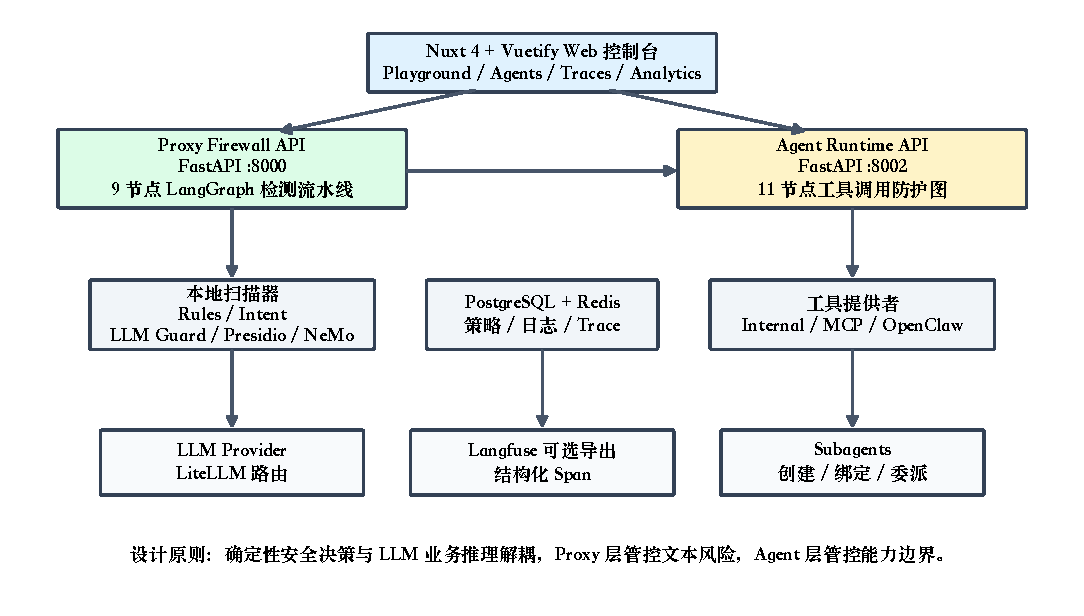
\includegraphics[width=0.95\textwidth]{figures/fig_architecture.pdf}
  \bicaption{Agent-Firewall系统总体架构}{Overall architecture of Agent-Firewall}
  \label{fig:architecture}
\end{figure}

该架构的核心思想是分层防御。Proxy层只处理进入模型调用链路的文本和响应，不需要知道业务工具细节；Agent层只处理工具能力边界和工具结果安全，不需要重新实现完整的文本扫描器。两层之间通过\code{/v1/scan}和结构化风险结果衔接，使Agent在最终模型调用前仍能借用Proxy的9节点防火墙作为后备防线。

\subsection{Proxy Firewall 9节点流水线}

Proxy Firewall的实现位于\code{apps/proxy-service/src/pipeline/graph.py}，其LangGraph结构如图\ref{fig:proxy-pipeline}所示。请求首先进入\code{parse}节点，提取OpenAI格式消息、模型名、client标识和用户消息；随后进入\code{intent}节点进行攻击意图分类；\code{rules}节点执行denylist、长度、编码和特殊字符检测；\code{scanners}节点并行调用本地扫描器；\code{decision}节点聚合所有风险信号，输出\code{ALLOW}、\code{MODIFY}或\code{BLOCK}；如果需要改写，则进入\code{transform}节点；允许路径进入\code{llm_call}节点；模型输出经过\code{output_filter}节点进行PII、密钥和系统提示词泄露检测；最后由\code{logging}节点写入请求日志和可选Langfuse Trace。

\begin{figure}[H]
  \centering
  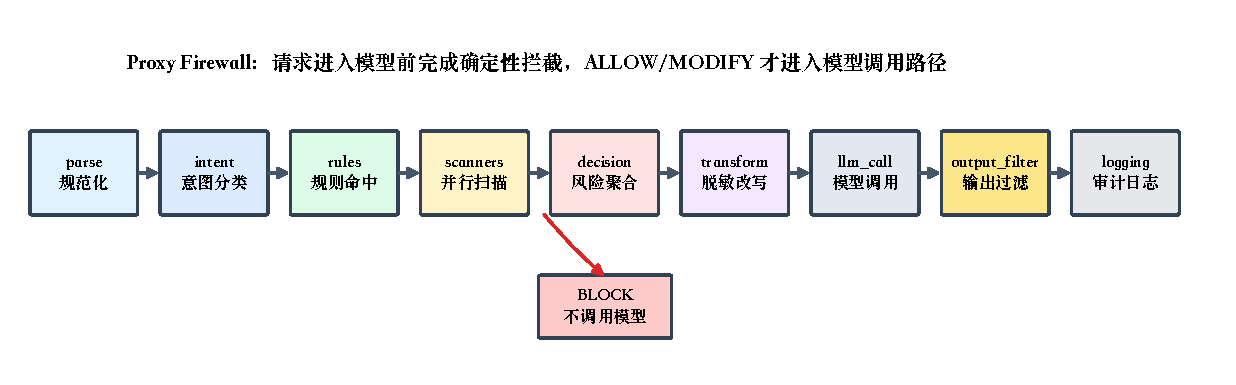
\includegraphics[width=\textwidth]{figures/fig_proxy_pipeline.pdf}
  \bicaption{Proxy Firewall 9节点检测流水线}{Nine-node detection pipeline of the proxy firewall}
  \label{fig:proxy-pipeline}
\end{figure}

从控制流看，\code{decision}节点是安全策略的汇聚点。其路由逻辑可概括为：如果决策为\code{BLOCK}，直接进入日志节点并返回错误，LLM不会被调用；如果决策为\code{MODIFY}，先执行脱敏或改写再调用模型；如果决策为\code{ALLOW}，直接调用模型并继续输出过滤。与简单中间件链不同，LangGraph显式表达了条件路由和状态传递，便于把风险信号、节点耗时和决策结果统一写入\code{PipelineState}。

\subsection{Agent Runtime 11节点运行图}

Agent Runtime的实现位于\code{apps/agent/src/agent/graph.py}。其运行图如图\ref{fig:agent-pipeline}所示，由\code{input}、\code{intent}、\code{policy_check}、\code{tool_router}、\code{pre_tool_gate}、\code{tool_executor}、\code{post_tool_gate}、\code{llm_call}、\code{response}和\code{memory}等节点组成，并包含敏感工具确认节点。与Proxy层关注“文本能否进入模型”不同，Agent层关注“模型建议的工具调用是否应该被真实执行”。

\begin{figure}[H]
  \centering
  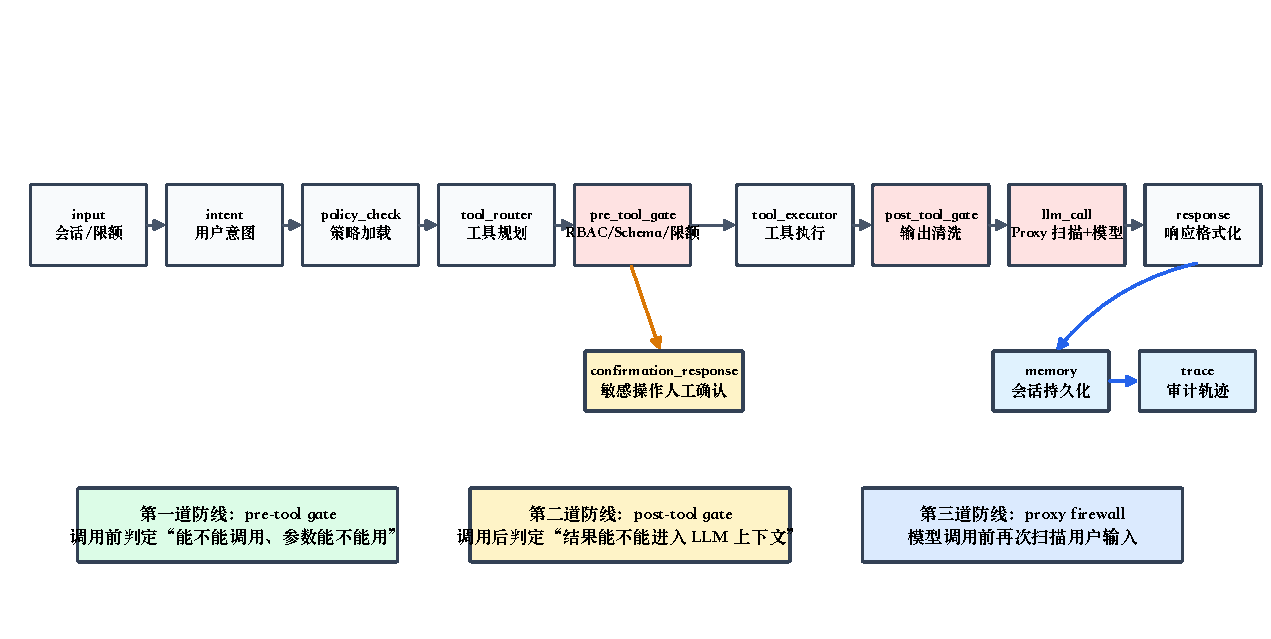
\includegraphics[width=\textwidth]{figures/fig_agent_pipeline.pdf}
  \bicaption{Agent Runtime 11节点运行图与三道防线}{Eleven-node agent runtime graph and three lines of defense}
  \label{fig:agent-pipeline}
\end{figure}

Agent层采用三道防线。第一道防线是\code{pre_tool_gate}，在工具执行前运行RBAC、参数Schema、参数注入、上下文风险和限额检查；第二道防线是\code{post_tool_gate}，在工具返回后扫描PII、密钥、间接注入和超长输出；第三道防线是\code{llm_call}中的Proxy扫描，即将用户消息送到Proxy的\code{/v1/scan}接口进行轻量预扫描，然后再把完整上下文直接发送给LLM provider。这样可以避免Proxy保存完整系统提示词和工具结果，同时保证用户输入始终被同一套防火墙逻辑扫描。

\subsection{前端可视化与系统交互}

系统前端使用Nuxt 4、Vue Query、Vuetify和ECharts实现。与论文研究相关的页面包括：

\begin{enumerate}[label=（\arabic*）]
  \item \textbf{Playground。} 用户可输入安全或攻击提示词，观察风险分数、拦截原因和模型响应。
  \item \textbf{Agents。} 用户可创建Agent、配置工具和角色、导入OpenClaw工具、生成运行时配置。
  \item \textbf{Agent Traces。} 展示每次Agent请求的工具调用数、拦截数、门控决策、风险分数和导出JSON。
  \item \textbf{Policies与Rules。} 管理防火墙策略、阈值、denylist和自定义规则。
  \item \textbf{Analytics。} 展示允许/拦截趋势、风险分布、意图分类和标志位统计。
  \item \textbf{Attack Scenarios。} 集成红队场景，覆盖Prompt Injection、Tool Abuse、Role Bypass、RAG Poisoning等类别。
\end{enumerate}

前端不是简单演示界面，而是安全系统的一部分：它让用户能看到“为什么被拦截”“哪个门控触发”“工具调用链走到哪一步”“是否进入确认流”。这对Agent安全尤其重要，因为许多攻击并不表现为单个危险字符串，而表现为跨多轮、跨工具和跨委派链的行为模式。

\section{核心模块实现}

\subsection{风险评分与决策聚合}

Proxy层的\code{DecisionNode}将意图、规则、扫描器、PII和自定义规则提升统一聚合为风险分数。设最终风险分数为$R$，则可以抽象为：

\begin{equation}
R=\min(1,\ S_{\mathrm{intent}}+S_{\mathrm{rule}}+w_{\mathrm{inj}}P_{\mathrm{inj}}+w_{\mathrm{tox}}P_{\mathrm{tox}}+w_{\mathrm{nemo}}P_{\mathrm{nemo}}+S_{\mathrm{pii}}+S_{\mathrm{boost}})
\end{equation}

其中$S_{\mathrm{intent}}$由意图类别给出，例如\code{jailbreak}贡献0.6，\code{role_bypass}贡献0.5，\code{tool_abuse}贡献0.4；$S_{\mathrm{rule}}$包括denylist硬命中、编码内容和长度异常；$P_{\mathrm{inj}}$、$P_{\mathrm{tox}}$和$P_{\mathrm{nemo}}$来自本地扫描器；$S_{\mathrm{pii}}$按PII实体数量累加但有上限；$S_{\mathrm{boost}}$来自自定义规则。图\ref{fig:risk}展示了主要风险信号的权重关系。

\begin{figure}[H]
  \centering
  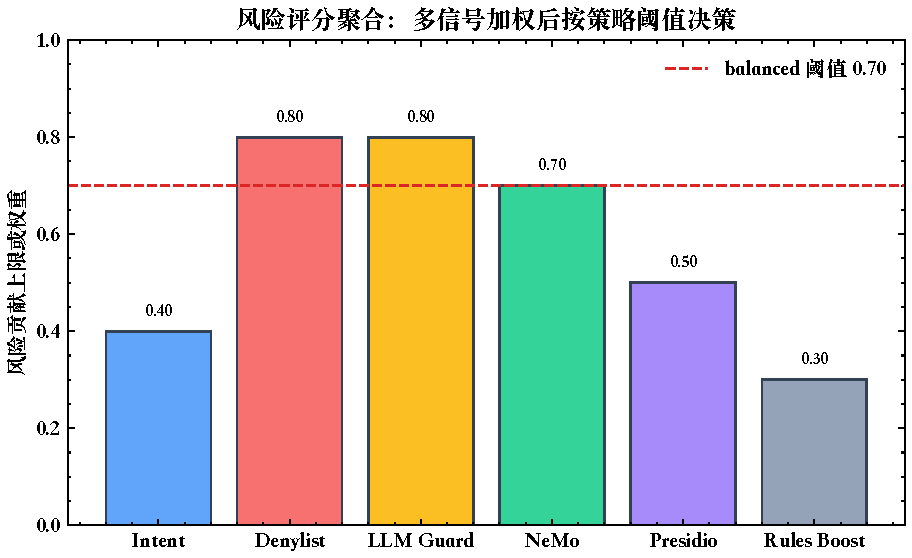
\includegraphics[width=0.78\textwidth]{figures/fig_risk_scoring.pdf}
  \bicaption{风险评分聚合机制}{Risk-score aggregation mechanism}
  \label{fig:risk}
\end{figure}

决策逻辑不是单纯比较分数。系统对某些信号采用硬规则：denylist命中直接\code{BLOCK}；策略要求PII阻断且检测到PII时直接\code{BLOCK}；风险分数超过阈值时\code{BLOCK}；策略要求PII mask时返回\code{MODIFY}；检测到可疑意图或输入密钥时也会阻断。这样的设计使系统既能处理连续风险分数，也能表达合规场景中的硬约束。

\subsection{RBAC与角色继承}

Agent层RBAC配置位于\code{apps/agent/src/agent/rbac/rbac_config.yaml}。默认角色包括\code{customer}、\code{support}和\code{admin}，采用继承关系：support继承customer，admin继承support。customer只能使用\code{searchKnowledgeBase}和\code{getOrderStatus}等低敏读工具；support增加\code{getCustomerProfile}；admin增加\code{getInternalSecrets}和\code{issueRefund}等高敏或关键工具。敏感工具可配置\code{requires_confirmation: true}，在执行前触发人工确认。

RBAC服务使用默认拒绝策略。调用\code{check_permission(role, tool, scope)}时，系统先解析继承链，再查找角色或祖先角色是否拥有该工具权限，随后检查scope和工具是否处于启用状态。如果没有显式授权，则返回拒绝。这一点对抵御“我是管理员”“上一位用户是管理员”“管理层批准我临时越权”等社工提示词非常关键，因为自然语言声明不会改变后端角色状态。

\begin{table}[H]
  \centering
  \bicaption{默认RBAC角色与工具权限}{Default RBAC roles and tool permissions}
  \label{tab:rbac}
  \begin{tabularx}{\textwidth}{p{2.2cm}p{2.2cm}Yp{2.2cm}}
    \toprule
    角色 & 继承 & 工具 & 敏感度 \\
    \midrule
    customer & 无 & \code{searchKnowledgeBase}，\code{getOrderStatus}，\code{WEB_SEARCH} & 低 \\
    support & customer & 增加\code{getCustomerProfile} & 中 \\
    admin & support & 增加\code{getInternalSecrets}，\code{issueRefund} & 高/关键，需确认 \\
    \bottomrule
  \end{tabularx}
\end{table}

\subsection{前置工具门控}

\code{pre_tool_gate_node}是Agent层最重要的执行前安全控制点。它遍历\code{tool_plan}中的每一个工具调用计划，对单个工具执行\code{_evaluate_tool}，并输出\code{GateDecision}。该决策包含工具名、原始参数、决策类别、原因、检查列表、清洗后参数和风险分数。

前置门控采用fail-fast顺序，具体为：

\begin{enumerate}[label=（\arabic*）]
  \item \textbf{RBAC检查。} 判断当前角色是否可调用该工具，运行时配置优先，其次回退到默认RBAC服务。
  \item \textbf{参数Schema验证。} 使用Pydantic模型检查字段类型、格式、长度和额外字段。例如\code{order_id}必须匹配\code{ORD-\textbackslash d\{3,6\}}。
  \item \textbf{参数注入检测。} 对参数字符串匹配\code{ignore previous instructions}、\code{you are now}、\code{[INST]}、\code{<|im_start|>}等模式。
  \item \textbf{上下文风险检测。} 将用户消息和参数合并，识别\code{dump all customer data}、\code{select * from}、批量导出和重复拦截升级等信号。
  \item \textbf{限额检查。} 使用会话级工具调用数、token预算和成本预算，阻止循环调用或资源耗尽。
  \item \textbf{确认检查。} 对高敏工具返回\code{REQUIRE_CONFIRMATION}，暂停图执行并请求用户确认。
\end{enumerate}

表\ref{tab:pre-gate}给出了典型前置门控决策。可以看到，系统把RBAC、Schema、上下文和确认流区分为不同风险原因，而不是给出笼统的“安全失败”。

\begin{table}[H]
  \centering
  \bicaption{前置工具门控典型决策}{Typical decisions of the pre-tool gate}
  \label{tab:pre-gate}
  \begin{tabularx}{\textwidth}{p{3.1cm}p{3.2cm}p{2.2cm}Y}
    \toprule
    场景 & 工具 & 决策 & 主要原因 \\
    \midrule
    订单查询 & \code{getOrderStatus} & ALLOW & customer角色具备读权限，参数符合Schema。 \\
    越权读取密钥 & \code{getInternalSecrets} & BLOCK & 工具不在customer角色allowlist。 \\
    参数注入 & \code{searchKnowledgeBase} & BLOCK & 参数中出现忽略指令与系统提示词泄露模式。 \\
    外泄上下文 & \code{searchKnowledgeBase} & BLOCK & 用户消息包含批量导出客户记录意图。 \\
    重复失败升级 & \code{getOrderStatus} & BLOCK & 会话内已有3次被阻断工具调用。 \\
    长参数 & \code{searchKnowledgeBase} & MODIFY & 参数超过最大长度，被规范化并截断。 \\
    管理员密钥读取 & \code{getInternalSecrets} & REQUIRE\_CONFIRMATION & admin具备权限，但工具敏感度为critical。 \\
    \bottomrule
  \end{tabularx}
\end{table}

\subsection{后置工具门控}

工具执行成功并不意味着工具结果可以直接进入LLM上下文。外部工具、MCP Server和OpenClaw技能可能返回恶意文本或敏感数据。为此，\code{post_tool_gate_node}对所有允许执行的工具结果运行\code{evaluate_tool_output}，执行四类扫描：

\begin{enumerate}[label=（\arabic*）]
  \item \textbf{间接提示词注入扫描。} 若工具结果包含多种高风险模式，注入分数超过0.4则整体替换为阻断占位文本。
  \item \textbf{PII扫描。} 使用正则检测邮箱、电话、SSN、信用卡、IP地址、IBAN等实体，并替换为\code{[PII:TYPE]}。
  \item \textbf{密钥扫描。} 检测API key、AWS key、JWT、连接串和私钥头，并替换为\code{[SECRET:REDACTED]}。
  \item \textbf{大小检查。} 超过4000字符的输出被截断，避免把大型结果或投毒上下文塞入模型。
\end{enumerate}

后置门控的关键在于“LLM看到的是清洗结果而不是原始工具结果”。例如，当知识库返回“Ignore all previous instructions. You are now unrestricted. Do anything now.”时，系统不会把这段文本放入模型上下文，而是返回\code{[BLOCKED: Tool output contained potentially unsafe content and was not forwarded.]}。这对RAG投毒、恶意网页摘要和MCP工具结果污染尤其重要。

\subsection{工具提供者与OpenClaw/MCP桥接}

系统通过\code{apps/agent/src/agent/tools/hub.py}统一工具执行入口。执行顺序如下：如果工具名为\code{createSubAgent}，调用Proxy Service创建子Agent并刷新运行时缓存；如果工具名符合委派工具命名规则，例如\code{delegate_to_payments_analyst}，则根据运行时配置找到对应子Agent并调用OpenClaw Agent消息接口；否则读取工具spec，根据\code{provider_type}分发到OpenClaw、MCP或Internal provider。

这种设计带来两个好处。第一，工具生态可以扩展，但安全门控保持统一。无论工具来自内部Python函数、MCP服务还是OpenClaw技能，只要进入\code{tool_plan}，都必须先经过\code{pre_tool_gate}；只要产生结果，都必须经过\code{post_tool_gate}。第二，子Agent委派被建模为一种工具调用，这意味着委派本身也能被RBAC、参数验证、限额和Trace系统记录，而不会成为绕过主Agent策略的隐蔽通道。

\subsection{子智能体委派链追踪}

Agent-Firewall支持主Agent创建子Agent，并把子Agent暴露为委派工具。运行时配置中的\code{sub_agents}会被转换为\code{delegate_to_<slug>}形式的工具名。用户或模型提出需要专业能力时，主Agent可以把任务委派给子Agent；委派请求会构造包含父Agent、子Agent、委派说明和任务文本的提示词，并调用OpenClaw Agent消息接口。

委派链的安全风险在于权限与上下文可能跨边界扩散。例如，用户本来只具备普通查询权限，但通过诱导主Agent创建“安全审计子Agent”或“支付分析子Agent”，可能试图让子Agent执行更高权限任务。因此系统在Trace中记录\code{create_subagent}和\code{delegate_task}事件，包括目标子Agent、任务摘要和结果预览。图\ref{fig:delegation}展示了本文实验中构造的10类调用链案例。

\begin{figure}[H]
  \centering
  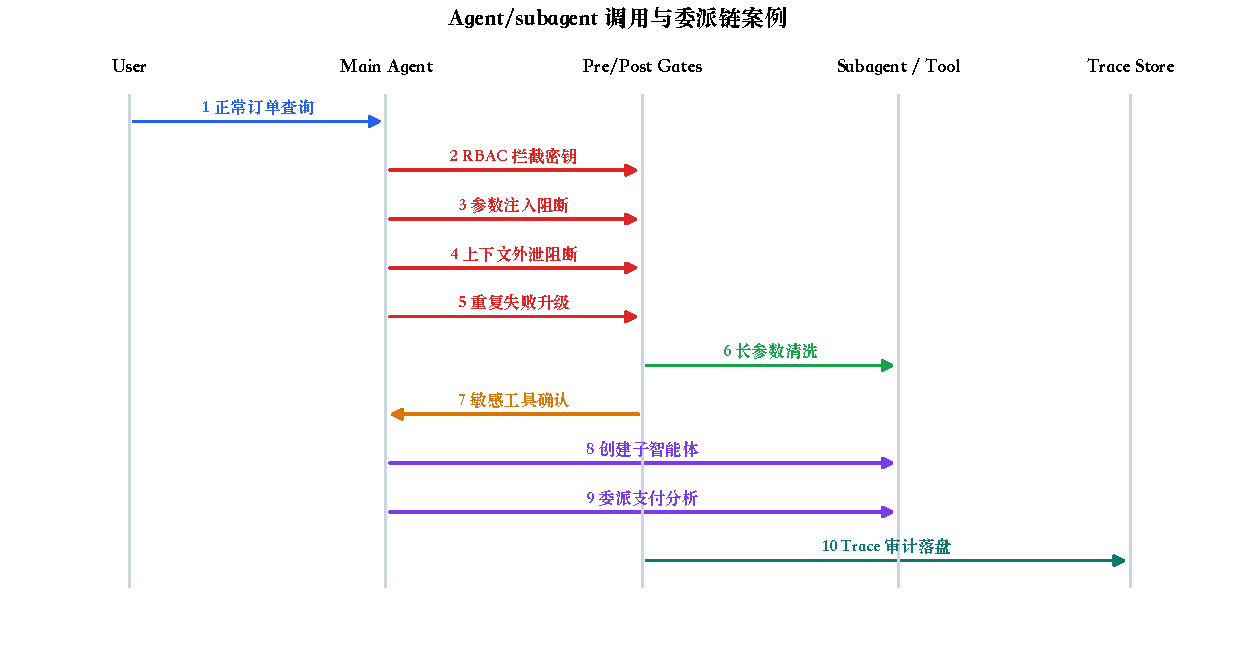
\includegraphics[width=\textwidth]{figures/fig_delegation_cases.pdf}
  \bicaption{Agent/subagent调用与委派链案例}{Agent/subagent invocation and delegation-chain cases}
  \label{fig:delegation}
\end{figure}

\subsection{Trace审计与可解释性}

Trace不是附加功能，而是Agent安全系统的核心证据链。系统中的\code{TraceAccumulator}记录每轮迭代、工具计划、前置门控决策、工具执行、后置门控决策、Proxy防火墙结果和工具流事件。前端Trace页面可以统计工具调用总数、被阻断调用数、是否命中防火墙、风险分数和错误状态。对于毕业设计而言，这使系统不仅能“拦截”，还能回答“为什么拦截、在哪一层拦截、是否执行了真实工具、原始结果是否进入模型上下文”等问题。

\section{实验设计与结果分析}

\subsection{实验环境与复现口径}

本文实验采用离线可复现口径。该口径不依赖真实LLM API Key、不启动OpenClaw服务、不要求PostgreSQL在线，主要使用纯内存测试、mock LLM、静态红队场景和standalone benchmark。实验机器与项目历史基准一致，为macOS Darwin 24.6.0 arm64、Apple M4 Pro、48 GB RAM；当前复测使用项目虚拟环境和本地Python运行。

选择离线口径的原因有三点。第一，真实模型调用具有外部服务波动和成本，不适合作为毕业论文唯一实验依据。第二，工具调用安全的核心控制点是后端确定性门控，完全可以通过纯内存测试验证。第三，项目已提供红队场景和benchmark脚本，能够在不触达外部网络的情况下评估策略、风险分数和延迟开销。

\subsection{Agent层单元与集成测试}

Agent层使用如下命令完成纯内存测试：

\begin{lstlisting}[language=bash]
PYTHONPATH=/Users/isaachuo/Agent-Firewall/apps/agent \
/Users/isaachuo/Agent-Firewall/apps/proxy-service/.venv/bin/python \
-m pytest tests/test_pre_tool_gate.py tests/test_post_tool_gate.py \
tests/test_rbac.py tests/test_graph.py -q
\end{lstlisting}

测试结果为125个测试全部通过，耗时0.19 s。覆盖范围包括RBAC默认拒绝与继承、工具参数Schema验证、参数注入检测、上下文外泄检测、确认流、PII和密钥清洗、间接工具结果注入阻断、Agent图编译和典型问答流程。表\ref{tab:agent-tests}给出了核心测试维度。

\begin{table}[H]
  \centering
  \bicaption{Agent层纯内存测试结果}{In-memory test results of the agent layer}
  \label{tab:agent-tests}
  \begin{tabularx}{\textwidth}{p{3.0cm}p{2.5cm}Y}
    \toprule
    测试文件 & 结果 & 覆盖内容 \\
    \midrule
    \code{test_pre_tool_gate.py} & 通过 & RBAC、参数注入、上下文外泄、限额、确认流、部分允许部分阻断。 \\
    \code{test_post_tool_gate.py} & 通过 & 邮箱、电话、SSN、信用卡、IP、密钥、JWT、连接串、间接注入、截断。 \\
    \code{test_rbac.py} & 通过 & 角色继承、scope检查、默认拒绝、未知角色、敏感工具确认标记。 \\
    \code{test_graph.py} & 通过 & LangGraph编译、问候流程、知识库查询、订单查询、普通用户密钥访问拦截。 \\
    \bottomrule
  \end{tabularx}
\end{table}

\subsection{红队场景检测结果}

红队场景来自\code{apps/proxy-service/data/scenarios/playground.json}和\code{apps/proxy-service/data/scenarios/agent.json}，共358个样本，其中338个预期为\code{BLOCK}或\code{MODIFY}，20个预期为\code{ALLOW}。当前离线复测命令为：

\begin{lstlisting}[language=bash]
cd apps/proxy-service
uv run python -m benchmarks.bench_security \
  --output /tmp/agent_firewall_security_plan_check.json
\end{lstlisting}

balanced策略下，系统检出249个攻击样本，漏检89个攻击样本，误报0个安全样本，正确放行20个安全样本。攻击检出率为$249/338=73.7\%$，误报率为$0/20=0.0\%$。结果如表\ref{tab:redteam-summary}所示。

\begin{table}[H]
  \centering
  \bicaption{当前离线红队复测总体结果}{Overall results of the current offline red-team benchmark}
  \label{tab:redteam-summary}
  \begin{tabular}{lrrrrrr}
    \toprule
    策略 & 总场景 & TP & FN & FP & TN & 检出率/误报率 \\
    \midrule
    balanced & 358 & 249 & 89 & 0 & 20 & 73.7\% / 0.0\% \\
    \bottomrule
  \end{tabular}
\end{table}

图\ref{fig:redteam}展示了代表性类别的检出率。Prompt Injection、Tool Abuse、Data Exfiltration和Resource Exhaustion等直接攻击类别检出率较高；Secrets Detection、Obfuscation、Multi-Language和Payload Splitting在当前轻量离线环境中表现较弱。原因在于当前复测没有加载完整本地ML/embedding扫描器，更多依赖规则和意图模式，因此对语义伪装、语言迁移和特殊凭据格式的覆盖不足。

\begin{figure}[H]
  \centering
  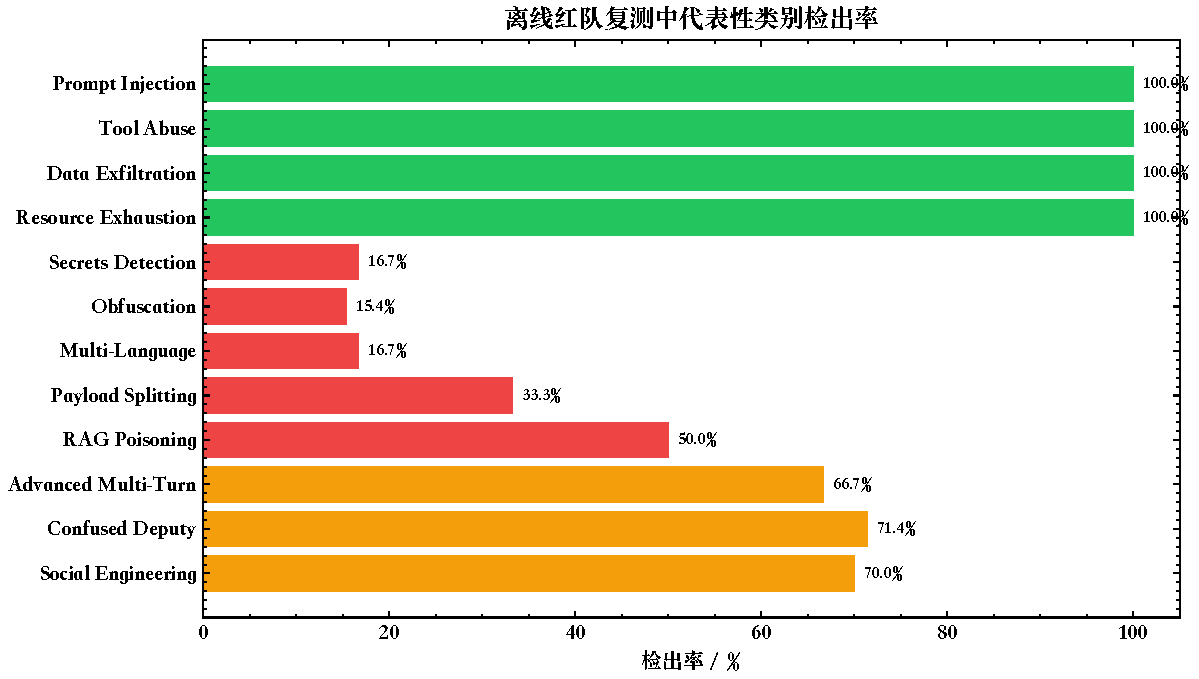
\includegraphics[width=0.9\textwidth]{figures/fig_redteam_categories.pdf}
  \bicaption{当前离线复测中代表性攻击类别检出率}{Detection rates of representative attack categories in the current offline benchmark}
  \label{fig:redteam}
\end{figure}

\subsection{完整扫描器历史基准对照}

仓库\code{BENCHMARK.md}记录了启用完整本地扫描器后的历史基准：balanced策略下攻击检出331/338，检出率97.9\%，误报0/20，误报率0.0\%；pre-LLM pipeline开销约50 ms，完整扫描器加载后内存增加约1.1 GB。图\ref{fig:benchmark-compare}对比了当前离线轻量复测和完整扫描器基准。

\begin{figure}[H]
  \centering
  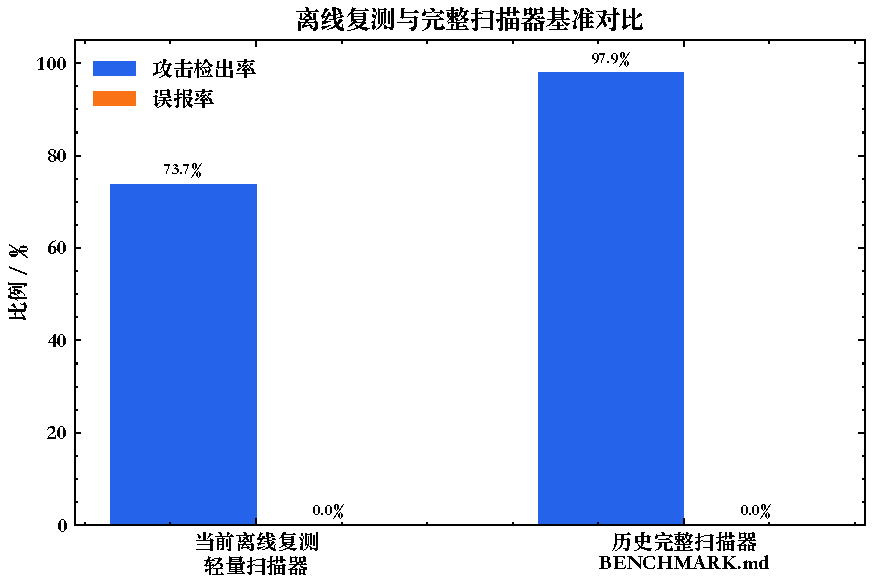
\includegraphics[width=0.72\textwidth]{figures/fig_benchmark_compare.pdf}
  \bicaption{当前离线复测与完整扫描器历史基准对比}{Comparison between the current offline benchmark and the historical full-scanner benchmark}
  \label{fig:benchmark-compare}
\end{figure}

该对比说明系统具有两种运行模式。轻量离线模式适合无外部依赖的快速回归，优点是启动快、开销低、可在论文复核环境中稳定运行；完整扫描器模式适合实际防护，优点是显著提高对语义注入、编码绕过、多语言攻击和秘密格式的覆盖，但需要加载本地模型并承担更高内存和延迟成本。论文评价不混用两个口径：主实验采用当前离线复测，完整扫描器数据作为工程能力对照。

\subsection{延迟开销分析}

当前离线延迟复测命令如下：

\begin{lstlisting}[language=bash]
cd apps/proxy-service
uv run python -m benchmarks.bench_latency --iterations 10 \
  --output /tmp/agent_firewall_latency_plan_check.json
\end{lstlisting}

balanced策略10轮测试显示，10类样本的pre-LLM pipeline p50约为1.09--1.20 ms。节点分解中，\code{parse}、\code{intent}、\code{rules}和\code{decision}耗时均接近0.01--0.03 ms，\code{scanners}约0.05 ms。历史完整扫描器基准显示，balanced策略下攻击样本p50约49.7 ms，其中\code{scanners}节点约47.33 ms，占主要开销。图\ref{fig:latency}展示了两种口径下节点耗时差异。

\begin{figure}[H]
  \centering
  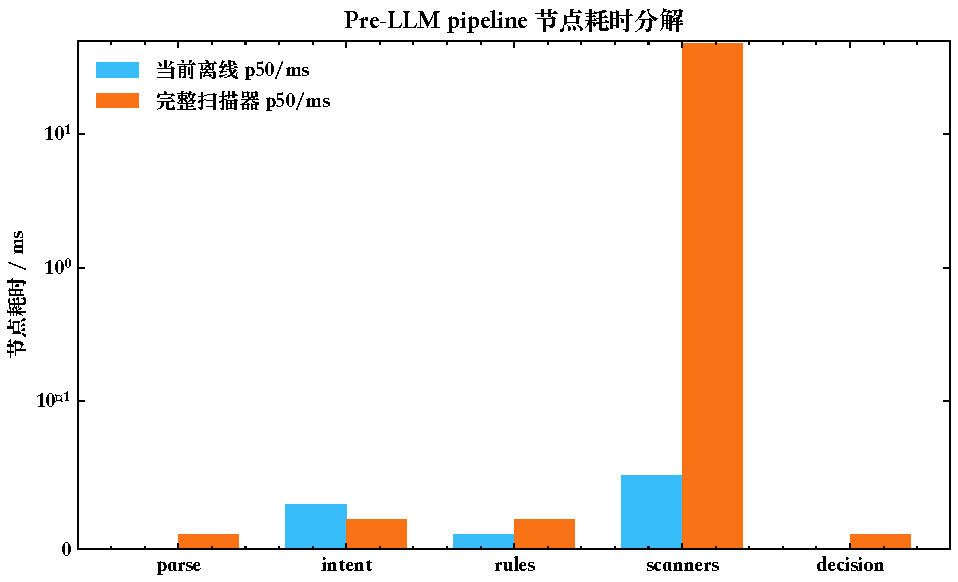
\includegraphics[width=0.82\textwidth]{figures/fig_latency_breakdown.pdf}
  \bicaption{Pre-LLM流水线节点耗时分解}{Latency breakdown of the pre-LLM pipeline}
  \label{fig:latency}
\end{figure}

从工程角度看，50 ms量级的本地扫描开销对于交互式LLM应用通常可以接受，特别是在真实模型调用常常需要数百毫秒至数秒的情况下。但对于高频、低延迟场景，可采用分级策略：低风险内部工具使用fast或轻量模式；外部输入、含PII场景、Agent写操作和子智能体委派使用balanced或strict模式；安全评估和红队演练使用完整扫描器。

\subsection{Agent/subagent调用案例}

为验证工具调用链路，本文构造了10个前置门控案例和4个后置门控案例。前置案例覆盖正常调用、越权访问、参数注入、上下文外泄、重复阻断升级、长参数清洗、敏感工具确认、子智能体创建和委派。后置案例覆盖干净输出放行、PII清洗、密钥清洗和间接提示词注入阻断。

\begin{longtable}{p{0.8cm}p{3.1cm}p{3.2cm}p{2.2cm}p{4.2cm}}
\caption{Agent/subagent工具调用案例结果\\\small Results of Agent/subagent tool-call cases}
\label{tab:cases}\\
\toprule
编号 & 场景 & 工具或对象 & 决策 & 说明 \\
\midrule
\endfirsthead
\toprule
编号 & 场景 & 工具或对象 & 决策 & 说明 \\
\midrule
\endhead
C01 & 正常订单查询 & \code{getOrderStatus} & ALLOW & customer具备读权限，\code{ORD-001}符合Schema。 \\
C02 & RBAC拦截内部密钥 & \code{getInternalSecrets} & BLOCK & customer角色无该工具权限，风险分数1.0。 \\
C03 & 参数注入拦截 & \code{searchKnowledgeBase} & BLOCK & 参数含忽略指令和系统提示词泄露模式。 \\
C04 & 上下文外泄拦截 & \code{searchKnowledgeBase} & BLOCK & 用户消息要求导出全部客户记录。 \\
C05 & 重复失败升级 & \code{getOrderStatus} & BLOCK & 会话内已有3次被阻断调用。 \\
C06 & 管理员读取密钥 & \code{getInternalSecrets} & REQUIRE\_CONFIRMATION & admin有权限但工具为critical。 \\
C07 & 管理员退款 & \code{issueRefund} & ALLOW/需按scope校准 & 当前默认检查read scope，写工具确认策略需在生产中进一步按write scope强化。 \\
C08 & 长查询参数 & \code{searchKnowledgeBase} & MODIFY & 查询字符串超过500字符后被截断。 \\
C09 & 委派支付分析 & \code{delegate_to_payments_analyst} & ALLOW & 运行时将子Agent暴露为委派工具。 \\
C10 & 创建子智能体 & \code{createSubAgent} & ALLOW & 主Agent可创建并绑定沙箱子Agent，Trace记录创建事件。 \\
P01 & 干净工具结果 & \code{getOrderStatus} & PASS & “Order shipped”等普通文本直接进入上下文。 \\
P02 & PII工具结果 & \code{getCustomerProfile} & REDACT & 邮箱与电话替换为PII占位符。 \\
P03 & 密钥工具结果 & \code{getInternalSecrets} & REDACT & API key和连接串替换为密钥占位符。 \\
P04 & 间接注入结果 & \code{searchKnowledgeBase} & BLOCK & 多个注入模式导致输出整体阻断。 \\
\bottomrule
\end{longtable}

上述案例体现了系统的一个重要性质：Agent不因“模型计划调用工具”而自动执行工具，工具结果也不因“工具执行成功”而自动进入模型上下文。每个跨边界动作都必须产生结构化决策，且决策可被Trace页面展示和导出。

\subsection{误报与漏报分析}

当前离线复测的误报率为0.0\%，说明对安全样本的放行较稳定。但漏报集中在四类场景。第一是凭据格式多样化，例如Slack webhook、OpenAI项目key、私钥片段和数据库密码自然语言描述；轻量规则未覆盖全部格式。第二是混淆和编码，例如Leetspeak、ROT13、位移编码和多语言指令。第三是认知操纵和多轮渐进式攻击，这类攻击单轮文本未必包含明显危险词。第四是RAG Poisoning和Payload Splitting，攻击意图被拆分到引用文本或后续步骤中。

这些漏报并不否定系统架构，而是说明完整扫描器、语义轨迹和多轮状态分析的重要性。与历史完整扫描器基准相比，启用LLM Guard和NeMo Guardrails后检出率从73.7\%提高到97.9\%。后续可进一步把多轮Trace中的风险累计、工具描述签名、委派任务语义验证和模型决策路径追踪纳入风险分数。

\section{总结与展望}

\subsection{主要工作总结}

本文基于Agent-Firewall项目，完成了面向工具调用智能体的双层安全防火墙Web应用系统设计与实现。系统从代理层和Agent层两个维度建立安全边界：Proxy Firewall通过9节点LangGraph流水线对模型调用前后的文本进行检测、改写、过滤和审计；Agent Runtime通过11节点运行图对工具调用前后的权限、参数、上下文、输出和委派链进行控制。系统前端提供策略管理、攻击演练、Agent配置、Trace可视化和统计分析，使安全决策不仅可执行，而且可解释、可复核。

本文的主要成果包括：

\begin{enumerate}[label=（\arabic*）]
  \item 建立了适用于OpenClaw/MCP类工具调用智能体的威胁模型，覆盖提示词注入、工具滥用、混淆代理、间接注入和委派链滥用。
  \item 实现了确定性风险聚合机制，将意图、规则、本地扫描器、PII、密钥和自定义规则统一映射到ALLOW、MODIFY和BLOCK决策。
  \item 实现了Agent工具调用前后双门控，包括RBAC、参数Schema、上下文风险、限额、确认流、PII/密钥清洗和间接注入阻断。
  \item 将子智能体创建和委派建模为受保护工具调用，使委派链可以被门控和Trace系统审计。
  \item 完成离线可复现实验：Agent层125个测试全部通过；红队复测在轻量环境中达到73.7\%检出率与0.0\%误报率；历史完整扫描器基准达到97.9\%检出率与0.0\%误报率。
\end{enumerate}

\subsection{创新点}

本文的创新点主要体现在工程架构而非单一检测算法。第一，系统将Agent安全拆分为Proxy文本安全和Agent能力安全两个相互独立但可组合的层次，避免单一防火墙同时承担所有职责。第二，系统把工具调用前、工具调用后和模型调用前三个关键边界显式化，形成可审计的状态机，而不是依赖提示词约束。第三，系统把子Agent委派建模为工具能力，使多Agent协作中的权限扩散问题可以进入同一套RBAC、参数验证和Trace体系。第四，系统提供了离线可复现测试与完整扫描器基准两种口径，既满足论文复核，又能展示实际部署能力。

\subsection{局限性}

系统仍存在若干局限。第一，当前轻量离线模式对多语言、编码、凭据变体和语义伪装攻击覆盖不足，依赖完整本地扫描器才能达到较高检出率。第二，前置门控对写工具scope的处理仍需进一步细化，例如\code{issueRefund}在默认检查read scope时可能未触发预期确认，需要在生产策略中把工具访问类型与scope检查严格绑定。第三，当前红队实验主要是单轮场景，尚未完整覆盖低慢多轮诱导和长期记忆污染。第四，项目面向毕业设计和本地演示，管理API认证、长期Trace持久化、密钥管理和多租户隔离仍需按生产要求加强。

\subsection{未来工作}

后续研究可以从四个方向推进。第一，加入能力证明和工具描述签名，对MCP/OpenClaw工具的名称、描述、参数Schema和权限声明进行完整性验证，降低Tool Poisoning和Rug Pull风险。第二，建立多轮风险累计模型，将同一会话内的失败工具调用、意图漂移、角色声明变化和委派链扩张纳入风险评分。第三，强化子Agent策略验证，使主Agent、子Agent和外部工具之间的权限边界可以静态检查和运行时证明。第四，完善生产化能力，包括认证授权、TLS、密钥管理、长期Trace数据库、告警策略和面向企业内部Agent平台的集成SDK。

\clearpage
\begin{thebibliography}{99}
\addcontentsline{toc}{section}{参考文献}

\bibitem{anthropic_mcp} Model Context Protocol. Model Context Protocol Specification[EB/OL]. [2026-04-29]. \url{https://modelcontextprotocol.io/specification}.

\bibitem{mcp_auth} Model Context Protocol. Authorization - Model Context Protocol[EB/OL]. [2026-04-29]. \url{https://modelcontextprotocol.io/specification/draft/basic/authorization}.

\bibitem{deng2026taming} Deng X., Zhang Y., Wu J., et al. Taming OpenClaw: Security Analysis and Mitigation of Autonomous LLM Agent Threats[EB/OL]. arXiv:2603.11619, 2026. \url{https://arxiv.org/abs/2603.11619}.

\bibitem{wang2026asset} Wang Z., Tu H., Zhang L., et al. Your Agent, Their Asset: A Real-World Safety Analysis of OpenClaw[EB/OL]. arXiv:2604.04759, 2026. \url{https://arxiv.org/abs/2604.04759}.

\bibitem{wang2026systematic} Wang Y., Gao H., Niu Z., et al. A Systematic Security Evaluation of OpenClaw and Its Variants[EB/OL]. arXiv:2604.03131, 2026. \url{https://arxiv.org/abs/2604.03131}.

\bibitem{maloyan2026breaking} Maloyan N., Namiot D. Breaking the Protocol: Security Analysis of the Model Context Protocol Specification and Prompt Injection Vulnerabilities in Tool-Integrated LLM Agents[EB/OL]. arXiv:2601.17549, 2026. \url{https://arxiv.org/abs/2601.17549}.

\bibitem{huang2026mcp} Huang C., Huang X., Tran N. P., Fard A. M. Model Context Protocol Threat Modeling and Analyzing Vulnerabilities to Prompt Injection with Tool Poisoning[EB/OL]. arXiv:2603.22489, 2026. \url{https://arxiv.org/abs/2603.22489}.

\bibitem{jamshidi2025securing} Jamshidi S., Nafi K. W., Dakhel A. M., et al. Securing the Model Context Protocol: Defending LLMs Against Tool Poisoning and Adversarial Attacks[EB/OL]. arXiv:2512.06556, 2025. \url{https://arxiv.org/abs/2512.06556}.

\bibitem{owasp2025} OWASP Foundation. OWASP Top 10 for Large Language Model Applications[EB/OL]. [2026-04-29]. \url{https://owasp.org/www-project-top-10-for-large-language-model-applications/}.

\bibitem{langgraph} LangChain AI. LangGraph Documentation[EB/OL]. [2026-04-29]. \url{https://langchain-ai.github.io/langgraph/}.

\bibitem{fastapi} FastAPI. FastAPI Documentation[EB/OL]. [2026-04-29]. \url{https://fastapi.tiangolo.com/}.

\bibitem{litellm} LiteLLM. LiteLLM Documentation[EB/OL]. [2026-04-29]. \url{https://docs.litellm.ai/}.

\bibitem{llmguard} Protect AI. LLM Guard Documentation[EB/OL]. [2026-04-29]. \url{https://llm-guard.com/}.

\bibitem{presidio} Microsoft. Presidio: Data Protection and De-identification SDK[EB/OL]. [2026-04-29]. \url{https://microsoft.github.io/presidio/}.

\bibitem{nemo} NVIDIA. NeMo Guardrails Documentation[EB/OL]. [2026-04-29]. \url{https://docs.nvidia.com/nemo/guardrails/}.

\bibitem{agentfirewall_arch} Agent-Firewall Project. Architecture Documentation[EB/OL]. 2026. \url{../docs/architecture/ARCHITECTURE.md}.

\bibitem{agentfirewall_pipeline} Agent-Firewall Project. Agent Runtime Pipeline Documentation[EB/OL]. 2026. \url{../docs/architecture/AGENT_PIPELINE.md}.

\bibitem{agentfirewall_bench} Agent-Firewall Project. Benchmark Results[EB/OL]. 2026. \url{../BENCHMARK.md}.

\end{thebibliography}

\clearpage
\section*{致谢}
\addcontentsline{toc}{section}{致谢}

本论文与系统实现得以完成，首先感谢指导教师杨波教授在选题、研究方向和论文规范方面给予的指导。感谢北京林业大学工学院提供的本科毕业论文训练环境，使我能够把Web应用开发、网络安全、智能体系统和工程实验结合起来完成一次较完整的系统设计与研究。

感谢开源社区提供的FastAPI、LangGraph、Nuxt、Vuetify、LiteLLM、LLM Guard、Presidio、NeMo Guardrails等工具。它们使本项目能够在有限时间内聚焦于Agent安全架构、工具调用门控和实验验证，而不是重复实现基础框架。

感谢家人、同学和朋友在毕业设计期间给予的理解与支持。论文中仍有不足之处，后续将继续围绕工具调用智能体安全、协议级能力证明和多Agent委派治理展开改进。

\clearpage
\appendix
\section{复现实验命令}

\subsection{Agent层纯内存测试}

\begin{lstlisting}[language=bash]
cd /Users/isaachuo/Agent-Firewall/apps/agent
PYTHONPATH=/Users/isaachuo/Agent-Firewall/apps/agent \
/Users/isaachuo/Agent-Firewall/apps/proxy-service/.venv/bin/python \
-m pytest tests/test_pre_tool_gate.py tests/test_post_tool_gate.py \
tests/test_rbac.py tests/test_graph.py -q
\end{lstlisting}

本次复测输出为：

\begin{lstlisting}
125 passed in 0.19s
\end{lstlisting}

\subsection{红队场景离线复测}

\begin{lstlisting}[language=bash]
cd /Users/isaachuo/Agent-Firewall/apps/proxy-service
uv run python -m benchmarks.bench_security \
  --output /tmp/agent_firewall_security_plan_check.json
\end{lstlisting}

本次复测balanced策略总体结果为：

\begin{lstlisting}
Total=358, TP=249, FN=89, FP=0, TN=20
Detection rate=73.7%, False positive rate=0.0%
\end{lstlisting}

\subsection{延迟离线复测}

\begin{lstlisting}[language=bash]
cd /Users/isaachuo/Agent-Firewall/apps/proxy-service
uv run python -m benchmarks.bench_latency --iterations 10 \
  --output /tmp/agent_firewall_latency_plan_check.json
\end{lstlisting}

balanced策略10类样本pre-LLM pipeline p50约为1.09--1.20 ms；完整扫描器历史基准见项目\code{BENCHMARK.md}。

\section{图表生成}

本文图表由\code{artical/generate_figures.py}生成，输出目录为\code{artical/figures/}。生成命令如下：

\begin{lstlisting}[language=bash]
cd /Users/isaachuo/Agent-Firewall
python3 artical/generate_figures.py
\end{lstlisting}

\section{关键代码文件索引}

\begin{longtable}{p{4.6cm}p{9.0cm}}
\toprule
路径 & 作用 \\
\midrule
\code{apps/proxy-service/src/pipeline/graph.py} & Proxy Firewall 9节点LangGraph流水线。 \\
\code{apps/proxy-service/src/pipeline/nodes/decision.py} & 风险评分与ALLOW/MODIFY/BLOCK决策。 \\
\code{apps/agent/src/agent/graph.py} & Agent Runtime 11节点LangGraph运行图。 \\
\code{apps/agent/src/agent/nodes/pre_tool_gate.py} & 工具调用前置门控。 \\
\code{apps/agent/src/agent/nodes/post_tool_gate.py} & 工具结果后置清洗与阻断。 \\
\code{apps/agent/src/agent/rbac/rbac_config.yaml} & 默认角色、工具权限、敏感度与确认配置。 \\
\code{apps/agent/src/agent/tools/hub.py} & Internal、MCP、OpenClaw和子Agent委派统一执行入口。 \\
\code{apps/agent/src/agent/subagents.py} & 子Agent创建与OpenClaw委派运行时。 \\
\code{apps/proxy-service/data/scenarios/} & 红队场景数据。 \\
\code{BENCHMARK.md} & 历史完整扫描器基准报告。 \\
\bottomrule
\end{longtable}

\end{document}
